% Last changes from 26/06/23 by Magdalena Glas 
\documentclass[11pt,a4paper,german,notitlepage]{report}


%\usepackage[applemac]{inputenc} %Kommentierung entfernen,falls Mac
\usepackage[utf8]{inputenc} %Windows, Linux
%\usepackage[ansinew]{inputenc} %TeXnicCenter kann leider kein UTF-8


%Umlaute
%\usepackage[english]{babel}
\usepackage[ngerman]{babel}


%einige Variablen definieren
\newcommand{\titelthema}{Thema der \\ Arbeit}
\newcommand{\authorname}{Vorname Name}
\newcommand{\authormail}{email@adresse.de}
\newcommand{\matrikelnr}{1234567}
\newcommand{\abgabedatum}{09. September 9999}
\newcommand{\betreuer}{Max Muster}
\newcommand{\arbeitstyp}{Bachelor-\textbackslash Masterarbeit \textbackslash Seminar}


%use for seminars with multiple authors
\newcommand{\authornameTwo}{Vorname Nachname}
\newcommand{\authornameThree}{Vorname Nachname}


%use for seminars with multiple authors, this will be shown in the footer, therefore change settings for \rfoot below
\newcommand{\authornames}{Meier, Müller and Huber}


% Standardschriftart
%\usepackage{times}
%\usepackage{garamond}

% Default-Schriften (\rmdefault Times, 
%\sfdefault Helvetica und \ttdefault Courier
%besser als \usepackage{times} da auch Mathematikschriften 
%berücksichtigt werden
\usepackage{mathptmx}  %Times
\usepackage[scaled=.92]{helvet}
%\usepackage{mathpazo} %Palatino
%\usepackage[scaled=.96]{berasans}
\usepackage{courier}

%Grafiken
\usepackage{graphicx}
\usepackage{subfigure} 

% Grafiken in einem Unterordner speichern
\graphicspath{{./images/}}

% Schöne Anführungszeichen
\usepackage{csquotes}


% Tabellen
\usepackage{tabularx}
\usepackage{booktabs}

%Supporting apa citation styl with round brackets
\usepackage[round]{natbib} 

% Seitenränder
\usepackage[a4paper]{geometry}
\geometry{top=26mm, bottom=19mm, left=50mm, right=25mm, includefoot}

% Seitenränder auf Deckblatt
\usepackage[strict]{changepage}

%Querseiten mit korrekter Kopf-/Fußzeile
\usepackage{pdflscape}


%sauberer Blocksatz, optischer Randausgleich
\usepackage{microtype}


%1,5facher Zeilenabstand nur im Fließtext
\usepackage{setspace}
\onehalfspacing

%einfaches Anpassen von Kopf- und Fußzeilen 
\usepackage{fancyhdr}

\rhead{\small\thepage}
\lhead{\footnotesize\leftmark}
\chead{}
\rfoot{\footnotesize{\authorname, \the\year}}
\lfoot{\footnotesize{\arbeitstyp}}
\cfoot{}

%für Seminare
%\rfoot{\footnotesize{\authornames, \the\year}}


% zusätzliche Sonderzeichen
%\usepackage{textcomp} 


% Mathematisches
%\usepackage{amssymb}
%\usepackage{amsmath} 
%\usepackage{amsfonts} 


% Code und Pseudocode
%\usepackage[ruled]{algorithm}
%\usepackage{algpseudocode}
%\usepackage[boxed]{algorithm}
%\usepackage{algpseudocode}

%Silbentrennung
\usepackage[T1]{fontenc}



% PDF options
\usepackage[hyperfootnotes=false, pdfpagelabels]{hyperref}
\urlstyle{rm}
\hypersetup{%
bookmarksopen={true},
%bookmarksopenlevel={2},
bookmarksnumbered=true,
pdfstartpage={1},
pdftitle={\arbeitstyp},
pdfsubject={\titelthema},
pdfauthor={\authorname},
pdfkeywords={},
pdfcreator={hyperref},
pdfproducer={LaTeX with hyperref},
pdffitwindow={false},
pdfpagelayout={OneColumn} %SinglePage
}


\usepackage{url}

\usepackage{color}
\usepackage{colortbl} %Für Listings
  \definecolor{dunkelgrau}{rgb}{0.7,0.7,0.7}
  \definecolor{hellgrau}{rgb}{0.9,0.9,0.9}

\usepackage{listing}
  \renewcommand{\listlistingname}{Quelltextverzeichnis}

\usepackage{listings}
  \lstset{numbers=left, numberstyle=\tiny, basicstyle=\scriptsize, backgroundcolor=\color{hellgrau}}
  \lstset{captionpos=b, aboveskip=15pt, belowskip=8pt, showstringspaces=false}



%Abkürzungsverzeichnis, nur verwendete Abkürzungen darstellen
\usepackage[printonlyused]{acronym}

%Anhang
\usepackage{appendix}


%Bild-, Tabellenuntschriften schöner formatieren
\usepackage[format=hang,margin=10pt,font=small,labelfont=bf]{caption}

%PDF einbinden
%\usepackage{pdfpages}
%\includepdf[pages=1-4]{Meindoku.pdf}


%Euro 
%\usepackage{eurosym} 
% das Euro-Zeichen kann so eingefügt werden: \euro{}

%Lorem ipsum Auto-Text um Format zu zeigen
\usepackage{blindtext}


% Trennlinie unter der Kopfzeile
\renewcommand{\plainheadrulewidth}{0.4pt}


% Abstand zwischen Absätzen
%\parskip 3pt

% kein Erstzeileneinzug
%\setlength{\parindent}{0em}

\author{
\authorname\\
\texttt{\authormail}
}

\begin{document}
%
%%%%%%%%%%%%%%%%%%%%%%%%%%%%%%%%%%%%%%%%%%%%%%%%%%%%%%%%%	
%
\pagenumbering{roman}


\phantomsection
%\addcontentsline{toc}{chapter}{Deckblatt}
\pdfbookmark[0]{Deckblatt}{Deckblatt}
\label{Deckblatt}

% Eidesstattliche Erklärung notwendig
%
%%%%%%%%%%%%%%%%%%%%%%%%%%%%%%%%%%%%%%%%%%%%%%%%%%%%%%%%%%%
%
% Deckblatt
%

\thispagestyle{empty}
\begin{titlepage}

%Seite zentrieren
\begin{adjustwidth}{-2cm}{}


\renewcommand{\thepage}{}

\begin{center}

\large{Universität Regensburg\\}

\large{Fakultät für Wirtschaftswissenschaften\\}

\large{\mbox{Lehrstuhl für Wirtschaftsinformatik I - Informationssysteme}}

\vspace*{5mm}

\Large{\textbf{\titelthema}}

\vspace*{5mm}

\includegraphics[width=0.55\textwidth]{Unisiegel.png}
%
\includegraphics[width=0.55\textwidth]{IFS_Logo.pdf}
\vspace*{4mm}

\Large{Bachelorarbeit}

\vspace*{5mm}


\end{center}
\begin{center}
Zur Erlangung des akademischen Grades "`Bachelor of Science (B.Sc.)"' im Studiengang\\
Wirtschaftsinformatik an der Fakultät für Wirtschaftswissenschaften der\\
Universität Regensburg

\vspace*{5mm}

\Large{Eingereicht bei: Prof. Dr. Günther Pernul\\}

\Large{Betreuung: \betreuer\\}

\end{center}

\vfill

\begin{center}
\large{Eingereicht am \abgabedatum\\}
\end{center}
\vspace*{0.6cm}
\begin{flushleft}
Eingereicht von:\\
\vspace*{7pt}
\authorname\\
Adresse\\
PLZ Ort\\
Matrikelnummer: \matrikelnr\\




\end{flushleft}

\end{adjustwidth}

\end{titlepage}

\newpage

%%%%%%%%%%%%%%%%%%%%%%%%%%%%%%%%%%%%%%%%%%%%%%%%%%%%%%%%%
%%% Ende Deckblatt

%
%%%%%%%%%%%%%%%%%%%%%%%%%%%%%%%%%%%%%%%%%%%%%%%%%%%%%%%%%%%
%
% Deckblatt
%

\thispagestyle{empty}
\begin{titlepage}


%Seite zentrieren
\begin{adjustwidth}{-2cm}{}


\renewcommand{\thepage}{}

\begin{center}

\large{Universität Regensburg\\}

\large{Fakultät für Wirtschaftswissenschaften\\}

\large{\mbox{Lehrstuhl für Wirtschaftsinformatik I - Informationssysteme}}

\vspace*{5mm}

\Large{\textbf{\titelthema}}

\vspace*{5mm}

\includegraphics[width=0.55\textwidth]{Unisiegel.png}
%
\includegraphics[width=0.55\textwidth]{IFS_Logo.pdf}
\vspace*{4mm}

\Large{Masterarbeit}

\vspace*{5mm}


\end{center}
\begin{center}
Zur Erlangung des akademischen Grades "`Master of Science (M.Sc.)"' im Studiengang\\
Wirtschaftsinformatik an der Fakultät für Wirtschaftswissenschaften der\\
Universität Regensburg

\vspace*{5mm}

\Large{Eingereicht bei: Prof. Dr. Günther Pernul\\}

\Large{Betreuung: \betreuer\\}

\end{center}

\vfill

\begin{center}
\large{Eingereicht am \abgabedatum\\}
\end{center}
\vspace*{0.6cm}
\begin{flushleft}
Eingereicht von:\\
\vspace*{7pt}
\authorname\\
Adresse\\
PLZ Ort\\
Matrikelnummer: \matrikelnr\\




\end{flushleft}

\end{adjustwidth}

\end{titlepage}

\newpage

%%%%%%%%%%%%%%%%%%%%%%%%%%%%%%%%%%%%%%%%%%%%%%%%%%%%%%%%%
%%% Ende Deckblatt



% Eidesstattliche Erklärung _nicht_ notwendig
\include{DeckblattPraxisseminar}
\include{DeckblattProjektseminar}
%
%%%%%%%%%%%%%%%%%%%%%%%%%%%%%%%%%%%%%%%%%%%%%%%%%%%%%%%%%%%
%
% Deckblatt
%

\thispagestyle{empty}
\begin{titlepage}


%Seite zentrieren
\begin{adjustwidth}{-2cm}{}


\renewcommand{\thepage}{}

\begin{center}

\large{Universität Regensburg\\}

\large{Fakultät für Wirtschaftswissenschaften\\}

\large{\mbox{Lehrstuhl für Wirtschaftsinformatik I - Informationssysteme}}

\vspace*{10mm}

\Large{\textbf{\titelthema}}

\vspace*{15mm}

\includegraphics[width=0.65\textwidth]{IFS_Logo.png}
\vspace*{15mm}

\Large{Seminararbeit}

\vspace*{10mm}



\Large{Eingereicht bei: Prof. Dr. Günther Pernul\\}

\Large{Betreuung: \betreuer\\}

\vspace*{5mm}

\large{Eingereicht am \abgabedatum\\}

\end{center}

\vfill

\begin{center}
\end{center}
\vspace*{6mm}
\begin{flushleft}
Eingereicht von:\\
\vspace*{7pt}
\authorname\\
Matrikelnummer: \matrikelnr\\




\end{flushleft}

\end{adjustwidth}

\end{titlepage}

\newpage

%%%%%%%%%%%%%%%%%%%%%%%%%%%%%%%%%%%%%%%%%%%%%%%%%%%%%%%%%
%%% Ende Deckblatt



%Abstract einbinden
\phantomsection
%\addcontentsline{toc}{chapter}{Abstract}
\pdfbookmark[0]{Abstract}{abstract}
\include{Abstract}

%%%%%%%%%%%%%%%%%%%%%%%%%%%%%%%%%%%%%%%%%%%%%%%%%%%%%%%%%


\newpage

% Keine Kopf-/Fußzeile auf den ersten Seiten
\pagestyle{fancyplain}

% "Kapitel" aus Kopfzeile weglassen
\renewcommand{\chaptermark}[1]{\markboth{\uppercase{\thechapter.\ #1}}{}}
% Nummerierungen nur bis Gliederungsebene 3 (\subsubsection)
\setcounter{secnumdepth}{3}
% Nur Überschriften bis Gliederungsebene 3 (\subsubsection) ins Inhaltsverzeichnis
\setcounter{tocdepth}{3}
\setcounter{page}{1}
\newpage


%Inhaltsverzeichnis
  \phantomsection
%  \addcontentsline{toc}{chapter}{Inhaltsverzeichnis}
  \pdfbookmark[0]{Inhaltsverzeichnis}{Inhaltsverzeichnis}
  \label{Inhaltsverzeichnis}
  \tableofcontents
  \newpage
  
%Abbildungsverzeichnis
  \clearpage
  \phantomsection
  \addcontentsline{toc}{chapter}{Abbildungsverzeichnis}
  \listoffigures
  \newpage

%Tabellenverzeichnis
  \clearpage
  \phantomsection
  \addcontentsline{toc}{chapter}{Tabellenverzeichnis}
  \listoftables
  \newpage

%Verzeichnis der Codelistings
  \clearpage
  \phantomsection
  \addcontentsline{toc}{chapter}{Listings}
  \lstlistoflistings
  \newpage

%Abkürzungsverzeichnis
% nur verwendete Abkürzungen werden dargestellt
  \clearpage
  \phantomsection
  \chapter*{Abkürzungsverzeichnis}
  \markboth{\uppercase{Abkürzungsverzeichnis}}{}
   \addcontentsline{toc}{chapter}{Abkürzungsverzeichnis}
   \begin{acronym}[MMMMMMMMM]
   %Kompaktansicht, Zeilenabstand verringern
   \setlength{\itemsep}{-\parsep}
   %Abkürzung fett
   \renewcommand*{\acsfont}[1]{{\textbf{#1}}}
   %auch für Abkürzungen Serifenschrift verwenden
   \renewcommand{\aclabelfont}[1]{\normalfont{\normalsize{#1}}\hfill}
      \acro{Bsp.}{Beispiel}
      \acro{SaaS}{Software as a Service}
      \acro{XML}{Extensible Markup Language}
   \end{acronym}
  \newpage

  \clubpenalty=10000
  \widowpenalty=10000 
  \displaywidowpenalty = 10000
  \tolerance=500 %Zeilenumbruch



%%%%%%%%%%%%%%%%%%%%%%%%%%%%%%%%%%%%%%%%%%%%%%%%%%%%%%%%%%%%%%%%%%%%%%%%%%

% Nummerierung wieder bei 1 beginnen
\setcounter{page}{1}

\pagestyle{fancy}
\pagenumbering{arabic}



%%%%%%%%%%%%%%%%%%%%%%%%%%%%%%% Einleitung %%%%%%%%%%%%%%%%%%%%%%%%%%%%%%%

%%%%%%%%%%%%%%%%%%%%%%%%%%%%%%%%% Einleitung %%%%%%%%%%%%%%%%%%%%%%%%%%%%%%%%%

\chapter{Einleitung}
\label{chap:Einleitung}

Lorem ipsum dolor sit amet, consetetur sadipscing elitr, sed diam nonumy eirmod tempor invidunt ut labore et dolore magna aliquyam erat, sed diam voluptua. At vero eos et accusam et justo duo dolores et ea rebum. Stet clita kasd gubergren, no sea takimata sanctus est Lorem ipsum dolor sit amet. Lorem ipsum dolor sit amet, consetetur sadipscing elitr, sed diam nonumy eirmod tempor invidunt ut labore et dolore magna aliquyam erat, sed diam voluptua. At vero eos et accusam et justo duo dolores et ea rebum. Stet clita kasd gubergren, no sea takimata sanctus est Lorem ipsum dolor sit amet.


%%%%%%%%%%%%%%%%%%%%%%%%%%%%%%%%%%%%%%%%%%%%%%%%%%%%%%%%%%%%%%%%%%%%%%%%%%%%%%


%%%%%%%%%%%%%%%%%%%%%%%%%%%%%%% Hauptteil %%%%%%%%%%%%%%%%%%%%%%%%%%%%%%%%

%%%%%%%%%%%%%%%%%%%%%%%%%%%%%%%%% Hauptteil %%%%%%%%%%%%%%%%%%%%%%%%%%%%%%%%%%

\chapter{Theoretischer Hintergrund}
\label{chap:background}

\section{Beispielkapitel}

\subsection{Referenzen und Fußnoten}

Dies ist eine Quellenangabe \citep{Pernul1994}. Man kann auch auf mehrere Arbeiten verweisen \citep{Pernul1994, pernul2009datenbanken}. Quellen werden in der Datei \textit{References.bib} gespeichert und können z.B. mit Mendeley\protect{\footnote{\url{https://www.mendeley.com}}} oder JabRef\protect{\footnote{\url{https://www.jabref.org/}}} verwaltet werden. Wenn etwas wörtlich zitiert werden soll, kann einfach
\textbf{\textbackslash enquote,} verwendet werden: \enquote{Dies ist ein Zitat}. So werden die Anführungszeichen immer richtig gesetzt. \par\smallskip


\subsection{Verwendung von Abkürzungen}

Die automatische Erstellung des Abkürzungsverzeichnisses ist ebenfalls sehr nützlich. Abkürzungen können in main.tex definiert werden. Zum Beispiel die Abkürzung \ac{SaaS}, wird so definiert, dass sie bei ihrer ersten Verwendung im Abkürzungsverzeichnis erscheint. Abkürzungen müssen konsistent verwendet werden, sobald sie eingeführt sind. Nicht jede Verwendung einer Abkürzung muss mit dem Befehl \verb+\ac{}+ verlinkt werden. Wenn jedoch viele Seiten zwischen der Verwendung einer Abkürzung liegen, kann ein Hyperlink für den Leser hilfreich sein.


\subsection{Aufzählungen}
In Latex gibt es zwei Arten von Aufzählungen, nummerierte Listen (\textbf{enumerate}):
\begin{enumerate}
    \item Punkt 1
    \item Punkt 2
    \item Punkt 3
\end{enumerate}

und umnummerierte Listen (\textbf{itemize}):

\begin{itemize}
    \item Punkt 1
    \item Punkt 2
    \item Punkt 3
\end{itemize}


\subsection{Abbildungen}
\label{sec:figures}

Die Größe von Abbildungen kann an die Textbreite angepasst werden. Abbildung~\ref{fig:Fig1} hat die volle Textbreite, Abbildung~\ref{fig:Fig2} 30\% davon.

\begin{figure} [!htb]
  \centering
  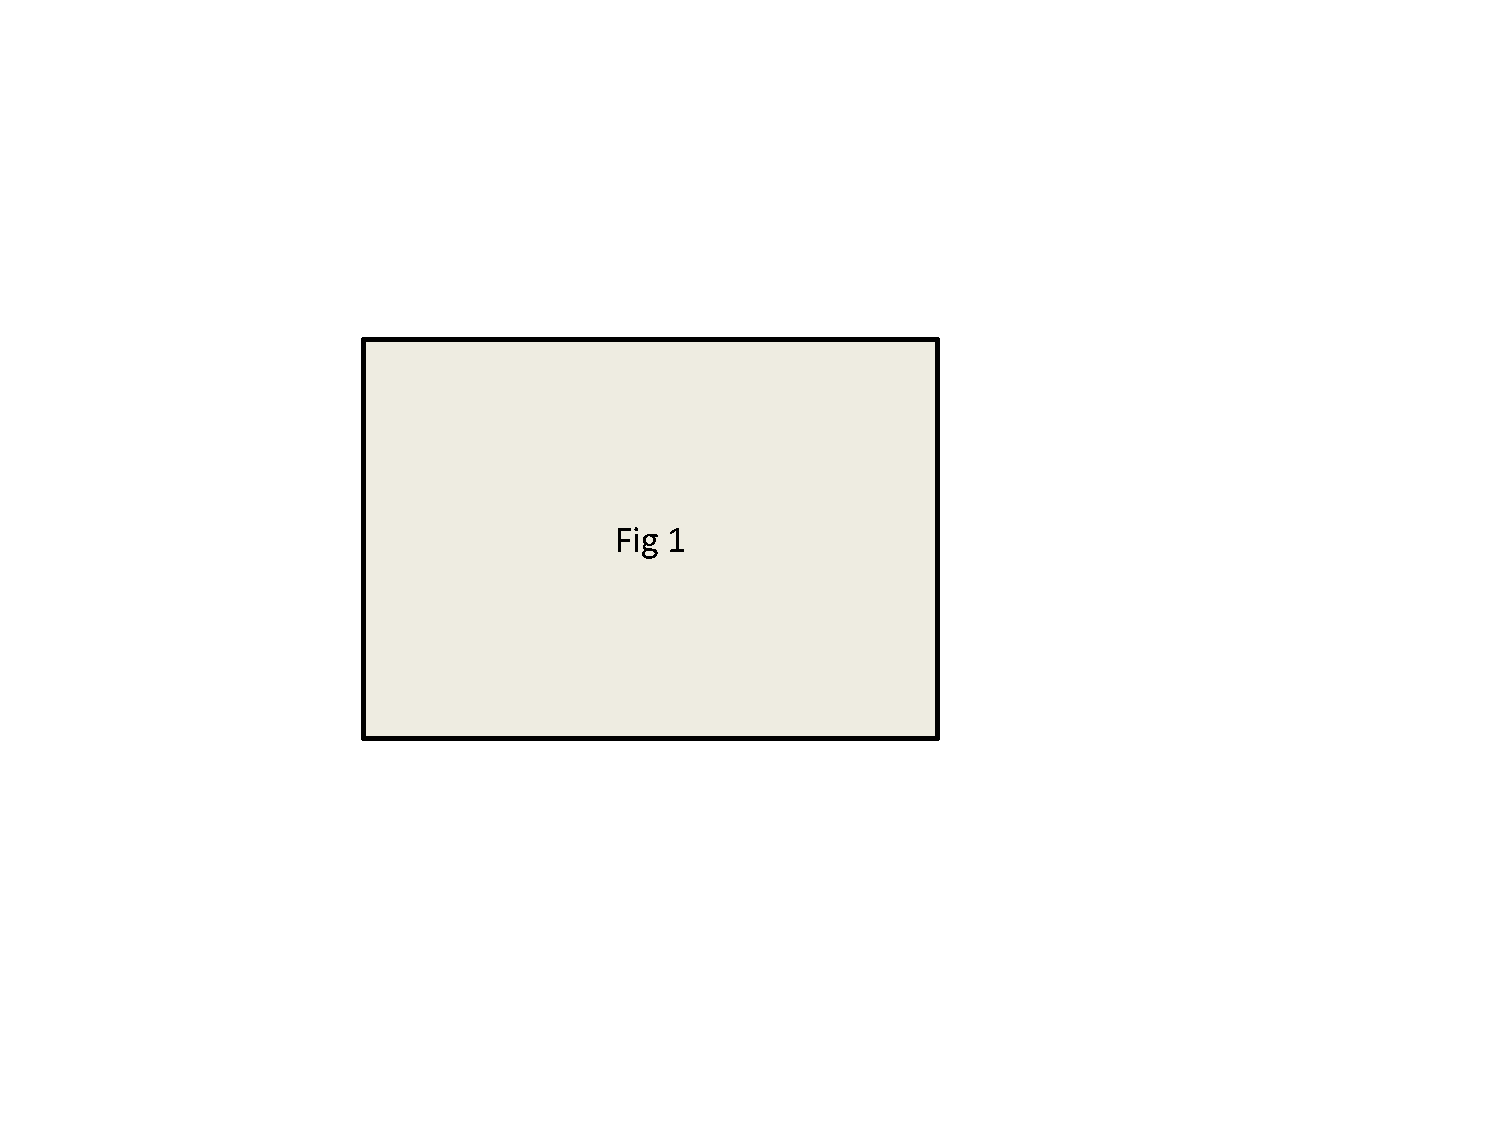
\includegraphics[width=\textwidth]{Fig1.pdf}
  \caption{Beispielhafte Abbildung.}
  \label{fig:Fig1}
\end{figure}


\begin{figure} [!htb]
  \centering
  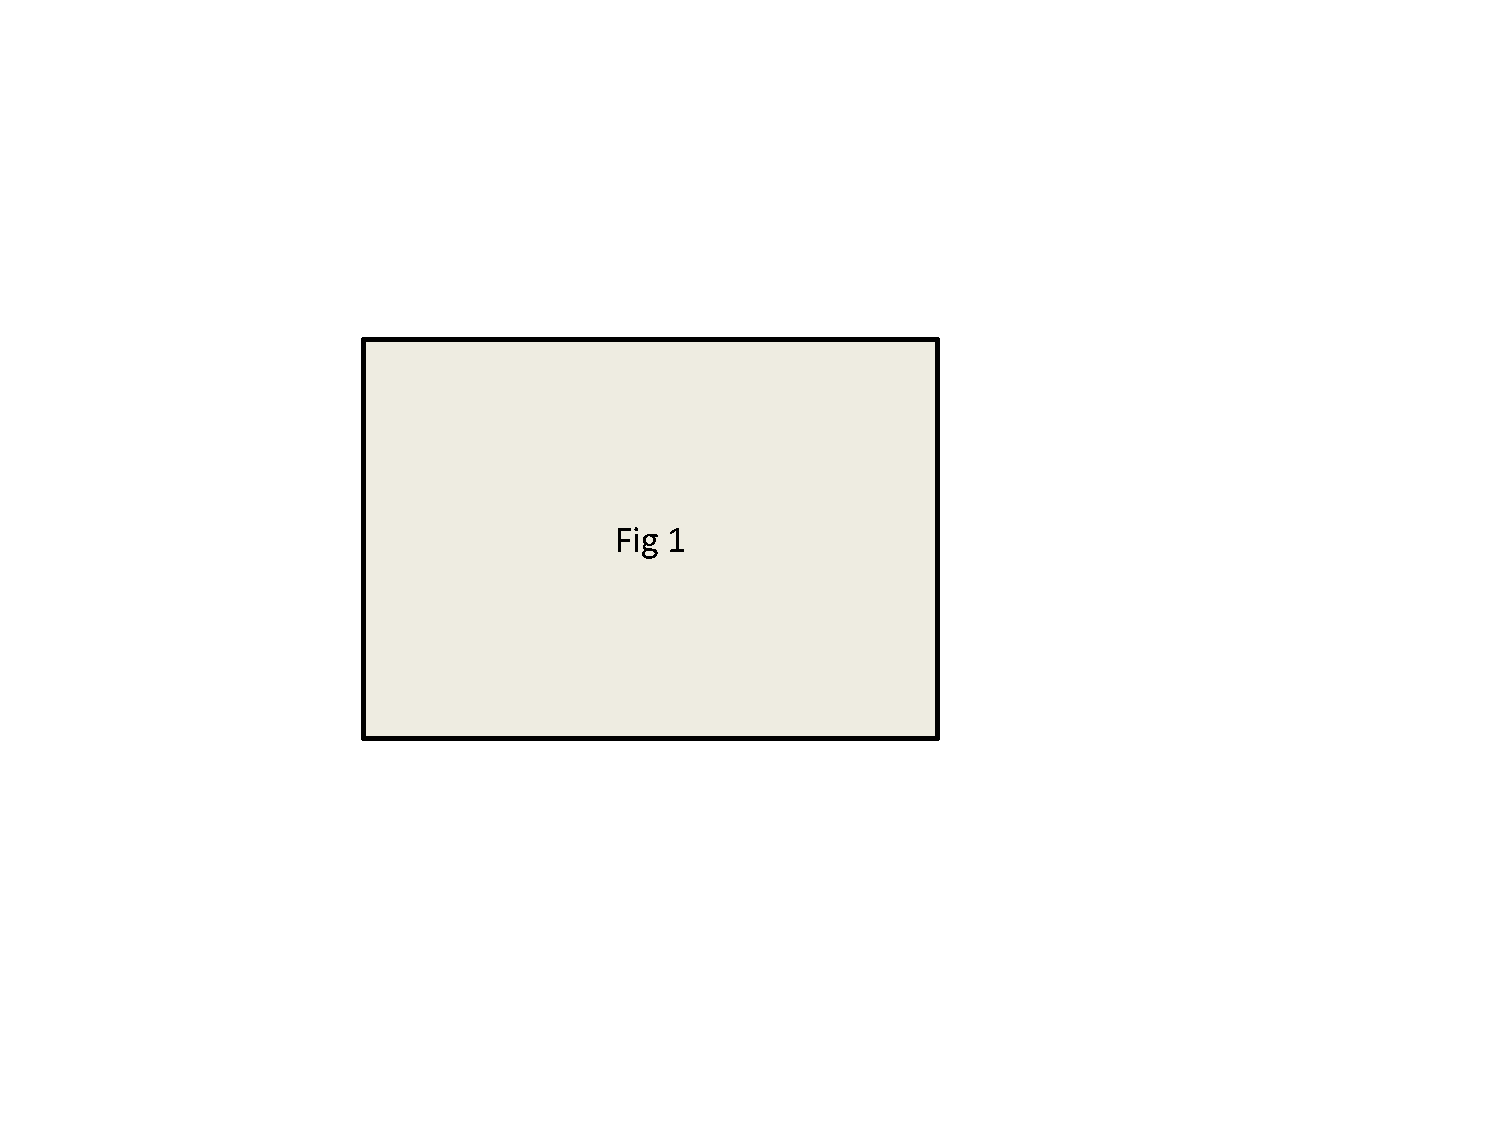
\includegraphics[width=0.3\textwidth]{Fig1.pdf}
 \caption{Beispielhafte kleinere Abbildung.}
  \label{fig:Fig2}
\end{figure}

\subsection{Tabellen}
\label{sec:tables}

In diesem Abschnitt ist ein Beispiel für eine Tabelle. Die Beschriftung von Tabellen befindet sich -- im Gegensatz zu Abbildungen -- immer oberhalb der Tabelle.

\begin{table} [h]
\centering
\caption{Beispielbeschriftung.}
\label{tab:feedback}
\begin{tabular}{lccc}
\toprule
\textbf{Bedingung} & \textbf{Mittelwert} & \textbf{Median} & \textbf{Standardabweichung} \\
\midrule
Wert 1 & 4.40 & 5 & 0.75 \\
Wert 2 & 4.35 & 4 & 0.72 \\
Wert 3 & 4.10 & 4 & 0.78 \\
Wert 4 & 4.23 & 4 & 0.72 \\
Wert 5 & 4.14 & 4 & 0.79 \\
\bottomrule
\end{tabular}
\end{table}








\subsection{Referenzen}

Der folgende Satz veranschaulicht die Verwendung von Referenzen. In Unterabschnitt~\ref{sec:figures}) wurde erklärt, wie man Abbildungen in \LaTeX verwendet, z. B. Abbildung~\ref{fig:Fig1}. Auf jede Tabelle, Abbildung oder Auflistung, die verwendet wird, muss mindestens einmal im Text Bezug genommen werden.

\subsection{Listings/Codebeispiele}

\lstset{language=JAVA, breaklines=true, tabsize=2}
\lstinputlisting[caption=HelloWorld,
label=lst:HelloWorld]{listings/HelloWorld.java}



\begin{landscape}

Seite im Querformat, z. B. für größere Abbildungen oder Tabellen; Fußzeile bleibt im Hochformat.

\end{landscape}




%%%%%%%%%%%%%%%%%%%%%%%%%%%%%%%%%%%%%%%%%%%%%%%%%%%%%%%%%%%%%%%%%%%%%%%%%%%%%%


%%%%%%%%%%%%%%%%%%%%%%%%%%%%%%%% Schluss %%%%%%%%%%%%%%%%%%%%%%%%%%%%%%%%%

%%%%%%%%%%%%%%%%%%%%%%%%%%%%%%%%%% Schluss %%%%%%%%%%%%%%%%%%%%%%%%%%%%%%%%%%%

\chapter{Schluss}
\label{chap:Schluss}

Lorem ipsum dolor sit amet, consetetur sadipscing elitr, sed diam nonumy eirmod tempor invidunt ut labore et dolore magna aliquyam erat, sed diam voluptua. At vero eos et accusam et justo duo dolores et ea rebum. Stet clita kasd gubergren, no sea takimata sanctus est Lorem ipsum dolor sit amet. Lorem ipsum dolor sit amet, consetetur sadipscing elitr, sed diam nonumy eirmod tempor invidunt ut labore et dolore magna aliquyam erat, sed diam voluptua. At vero eos et accusam et justo duo dolores et ea rebum. Stet clita kasd gubergren, no sea takimata sanctus est Lorem ipsum dolor sit amet.

%%%%%%%%%%%%%%%%%%%%%%%%%%%%%%%%%%%%%%%%%%%%%%%%%%%%%%%%%%%%%%%%%%%%%%%%%%%%%%


%%%%%%%%%%%%%%%%%%%%%%%%%%%%%%%%%%%%%%%%%%%%%%%%%%%%%%%%%%%%%%%%%%%%%%%%%%



%%%%%%%%%%%%%%%%%%%%%%%%% Literaturverzeichnis %%%%%%%%%%%%%%%%%%%%%%%%%%%

\newpage

\phantomsection
\addcontentsline{toc}{chapter}{Appendices}
\appendix
\appendixpage

%%\appendix
%%\phantomsection
%\renewcommand*\appendixpagename{Anhang} 
%%\appendixpage
%%\addappheadtotoc

\chapter{Erster Anhang}
\label{chap:anhang_1}

\chapter{Zweiter Anhang}
\label{chap:anhang_2}

\section{Anhang}
\label{sec:anhang_2_1}

\section{Anhang}
\label{sec:anhang_2_2}

\clearpage

%%%%%%%%%%%%%%%%%%%%%%%%% Literaturverzeichnis %%%%%%%%%%%%%%%%%%%%%%%%%%%
\phantomsection
\addcontentsline{toc}{chapter}{Literaturverzeichnis}
\bibliographystyle{apalike-german}
\bibliography{References}

\clearpage

%
%%%%%%%%%%%%%%%%%%%%%%%%%%%%%%%%%%%%%%%%%%%%%%%%%%%%%%%%%%%%%%%%%%%%%%%%%%
%% Eidesstattliche Erklärung %%%%
%
% nur bei Abschlussarbeiten!
%

\thispagestyle{empty}
\phantomsection
\label{erklaerung}
%\addcontentsline{toc}{chapter}{Erklärung}
\pdfbookmark[0]{Eidesstattliche Erklärung}{erklaerung}

\setlength{\parindent}{0em}

\markboth{\uppercase{Eidesstattliche Erklärung}}{}
\textbf{\large{Erklärung an Eides statt}}

\vspace*{65pt}

%% WICHTIG: unpassendes rauslöschen, sodass nur EINE Erklärung in der Arbeit steht 

%% Bachelor und Master nach Prüfungsordnung 2015
%\vspace*{20pt}
Ich habe die vorliegende Arbeit selbstständig verfasst und keine anderen als die angegebenen Quellen und Hilfsmittel benutzt. Die Arbeit wurde bisher an keiner anderen Hochschule zur Erlangung eines akademischen Grades eingereicht. Die vorgelegten Druckexemplare und die dem Prüfer / der Prüferin zur Verfügung gestellte elektronische Version (PDF-Datei) der Arbeit sind identisch. Von den in §13 Abs. 3 PO 2015 vorgesehenen Rechtsfolgen habe ich Kenntnis.

%% Bachelor nach Prüfungsordnung 2021
Ich habe die vorliegende Arbeit selbstständig verfasst und keine anderen als die angegebenen Quellen und Hilfsmittel benutzt. Die Arbeit wurde bisher an keiner anderen Hochschule zur Erlangung eines akademischen Grades eingereicht. Die vorgelegten Druckexemplare und die dem Prüfer / der Prüferin zur Verfügung gestellte elektronische Version (PDF-Datei) der Arbeit sind identisch. Von den in §27 Abs. 6 BPO 2021 vorgesehenen Rechtsfolgen habe ich Kenntnis.

\vspace*{65pt}

%% Master nach Prüfungsordnung 2021
Ich habe die vorliegende Arbeit selbstständig verfasst und keine anderen als die angegebenen Quellen und Hilfsmittel benutzt. Die Arbeit wurde bisher an keiner anderen Hochschule zur Erlangung eines akademischen Grades eingereicht. Die vorgelegten Druckexemplare und die dem Prüfer / der Prüferin zur Verfügung gestellte elektronische Version (PDF-Datei) der Arbeit sind identisch. Von den in §26 Abs. 6 MPO 2021 vorgesehenen Rechtsfolgen habe ich Kenntnis.


\vspace*{65pt}

Regensburg, den \abgabedatum

\vspace*{60pt}


\authorname

Matrikelnummer \matrikelnr

\end{document}
